\documentclass[10pt]{article}
\usepackage[letterpaper,text={6.5in,8.7in},centering]{geometry}
\usepackage{amssymb,amsmath,times,url,subfigure,graphicx,theorem,alltt,eepic,tikz}
%\usepackage[pdftex,urlcolor=blue,pdfpagemode=none,pdfstartview=FitH]{hyperref}

%% url smaller font.
\makeatletter
\def\url@leostyle{%
  \@ifundefined{selectfont}{\def\UrlFont{\sf}}{\def\UrlFont{\small\ttfamily}}}
\makeatother
\urlstyle{leo}

%\usepackage[all,import]{xy}

\newcommand{\norm}[1]{\ensuremath{\left\| #1 \right\|}}
\newcommand{\abs}[1]{\ensuremath{\left| #1 \right|}}
\newcommand{\bracket}[1]{\ensuremath{\left[ #1 \right]}}
\newcommand{\braces}[1]{\ensuremath{\left\{ #1 \right\}}}
\newcommand{\parenth}[1]{\ensuremath{\left( #1 \right)}}
\newcommand{\ip}[1]{\ensuremath{\langle #1 \rangle}}
\newcommand{\refeqn}[1]{(\ref{eqn:#1})}
\newcommand{\reffig}[1]{Fig. \ref{fig:#1}}
\newcommand{\tr}[1]{\mbox{tr}\ensuremath{\negthickspace\bracket{#1}}}
\newcommand{\deriv}[2]{\ensuremath{\frac{\partial #1}{\partial #2}}}
\newcommand{\SO}{\ensuremath{\mathrm{SO(3)}}}
\newcommand{\T}{\ensuremath{\mathrm{T}}}
\newcommand{\so}{\ensuremath{\mathfrak{so}(3)}}
\newcommand{\SE}{\ensuremath{\mathrm{SE(3)}}}
\newcommand{\se}{\ensuremath{\mathfrak{se}(3)}}
\renewcommand{\Re}{\ensuremath{\mathbb{R}}}
\renewcommand{\S}{\ensuremath{\mathbb{S}}}
\newcommand{\aSE}[2]{\ensuremath{\begin{bmatrix}#1&#2\\0&1\end{bmatrix}}}
\newcommand{\ase}[2]{\ensuremath{\begin{bmatrix}#1&#2\\0&0\end{bmatrix}}}
\newcommand{\D}{\ensuremath{\mathbf{D}}}
\newcommand{\pair}[1]{\ensuremath{\left\langle #1 \right\rangle}}
\newcommand{\met}[1]{\ensuremath{\langle\!\langle #1 \rangle\!\rangle}}
\newcommand{\Ad}{\ensuremath{\mathrm{Ad}}}
\newcommand{\ad}{\ensuremath{\mathrm{ad}}}
\newcommand{\g}{\ensuremath{\mathfrak{g}}}

\renewcommand{\baselinestretch}{1.2}
\date{}

\renewcommand{\thesubsection}{\arabic{subsection}. }
\renewcommand{\thesubsubsection}{\arabic{subsection}.\arabic{subsubsection} }

\theoremstyle{plain}\theorembodyfont{\normalfont}
\newtheorem{prob}{Problem}[section]
%\renewcommand{\theprob}{\arabic{section}.\arabic{prob}}
\renewcommand{\theprob}{\arabic{prob}}

\newenvironment{subprob}%
{\renewcommand{\theenumi}{\alph{enumi}}\renewcommand{\labelenumi}{(\theenumi)}\begin{enumerate}}%
{\end{enumerate}}%

\newenvironment{matlab}
{\begin{alltt}\small\renewcommand{\baselinestretch}{1.2}\selectfont}%
{\end{alltt}}

\newcommand*\circled[1]{%
  \tikz[baseline=(C.base)]\node[draw,circle,inner sep=0.5pt](C) {#1};\!
}

\begin{document}

\pagestyle{empty}
\section*{MAE3145: Simulating a Phasing Maneuver via STK}
\vspace*{-0.4cm}
\noindent{Due date: December 10, 2014}%\\%\vspace*{0.5cm}
\vspace*{0.2cm}


\begin{prob}
We discussed the following phasing maneuver in class. Consider an initial elliptic orbit $\circled{1}$ with the periapsis $A$ and the apoapsis $C$. There are chaser $A$ and target $B$ on the orbit. The initial true anomalies of the chaser and the target are given by $\theta_A=0$ and $\theta_B=90^\circ$, respectively. We designed a phasing orbit $\circled{2}$ of the chaser such that the chaser catches the target at the point $A$. 

\centerline{
\setlength{\unitlength}{1.2em}\centering\footnotesize
\begin{picture}(10,11)(-5,-4)
\put(0,0){\vector(1,0){5}}
\put(0,0){\vector(0,1){5.5}}
\put(0,0){\circle*{0.8}}
\put(3.4,0){\circle*{0.15}}\put(3.6,-0.6){$A$}
\put(0,4.5){\circle*{0.15}}\put(0.2,4.6){$B$}
\put(-6.8,0){\circle*{0.15}}\put(-7.5,-0.6){$C$}
\put(-5.7,0){\circle*{0.15}}\put(-6.4,-0.6){$D$}
\put(-1.7,0){\ellipse{10.2}{9.6}}
\put(-1.15,0){\ellipse{9.1}{6.8}}
\put(1.0,-2.1){\circled{2}}
\put(2.2,-3.9){\circled{1}}
\end{picture}}
\begin{align*}
r_A = 6800\,\mathrm{km},\quad r_C=13600\,\mathrm{km},\quad\theta_A=0,\quad\theta_B=90^\circ.
\end{align*}

We wish to simulate the resulting maneuver in STK according to the following steps.

\begin{enumerate}
\item Create a new scenario.
\item Insert the chaser satellite to the point $A$ of Orbit \circled{1}.
\begin{align*}
a_1 = \frac{1}{2}(r_A+r_C)=10200\,\mathrm{km},\quad e_1=\frac{r_C-r_A}{r_C+r_A}=0.3333,\quad i_1=0,\quad \omega_1=0,\quad\Omega_1=0,\quad \theta_A=0.
\end{align*}
\item Insert the target satellite to the point $B$ of Orbit \circled{1}.
\begin{align*}
a_1 = \frac{1}{2}(r_A+r_C)=10200\,\mathrm{km},\quad e_1=\frac{r_C-r_A}{r_C+r_A}=0.3333,\quad i_1=0,\quad \omega_1=0,\quad\Omega_1=0,\quad \theta_B=90^\circ.
\end{align*}
\item Take a snap shot of the resulting orbit at the 3D graphics window. \textbf{Save it as a jpg file, and upload it to Blackboard.} A sample jpg file is illustrated at the last page.


\item Double-click the chaser satellite at the left object browser, and change ``Propagator'' to ``Astrogator'' at the pull down menu. This requires that the orbital elements of the chaser should be \textbf{re-entered} at the following element tab of the initial state.

\centerline{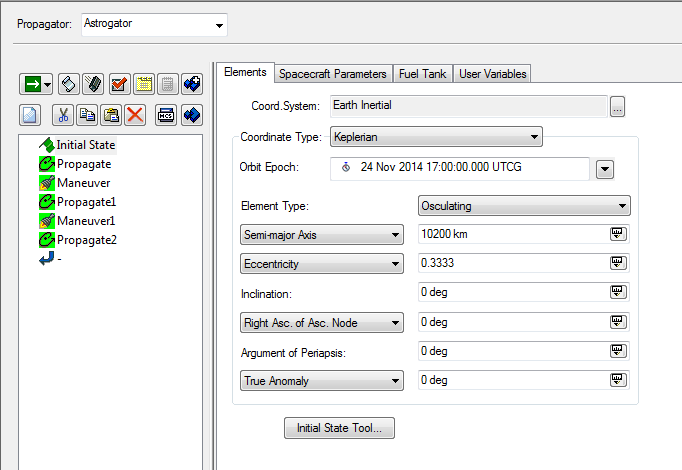
\includegraphics[width=0.7\textwidth]{Capture.eps}}


\item Describe the phasing maneuver of the chaser as follows:
\begin{itemize}
\item Propagate until periapsis before maneuver
\item First impulse $\Delta v_A = -0.2485\,\mathrm{km/s}$ to transfer the chaser to Orbit \circled{2}\\
(Choose ``AntiVelocity'' to enter a negative velocity change.)
\item Propagate until periapsis of Orbit \circled{2}
\item Second impulse $\Delta v_A = +0.2485\,\mathrm{km/s}$ to transfer the chaser to Orbit \circled{1}
\item Propagate until periapsis of Orbit \circled{1}
\end{itemize}

Choose ``Earth Point Mass'' for the type of propagator.

\centerline{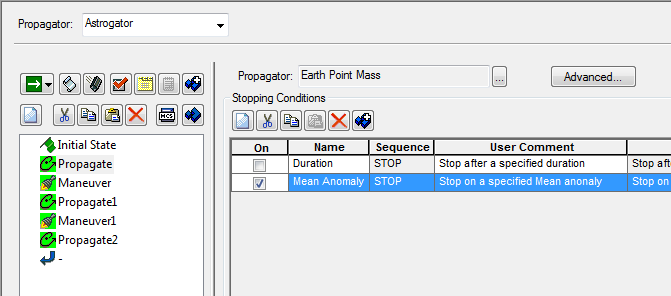
\includegraphics[width=0.7\textwidth]{Capture2.eps}}

\item Simulate the resulting maneuver at the 3D graphics window, and make it sure that the chaser catches the target.
\item Take a snap shot of the resulting orbit at the 3D graphics window. \textbf{Save it as a jpg file, and upload it to Blackboard.} A sample jpg file is illustrated at the next page.
\end{enumerate}

\end{prob}

\newpage

\begin{figure}
\centerline{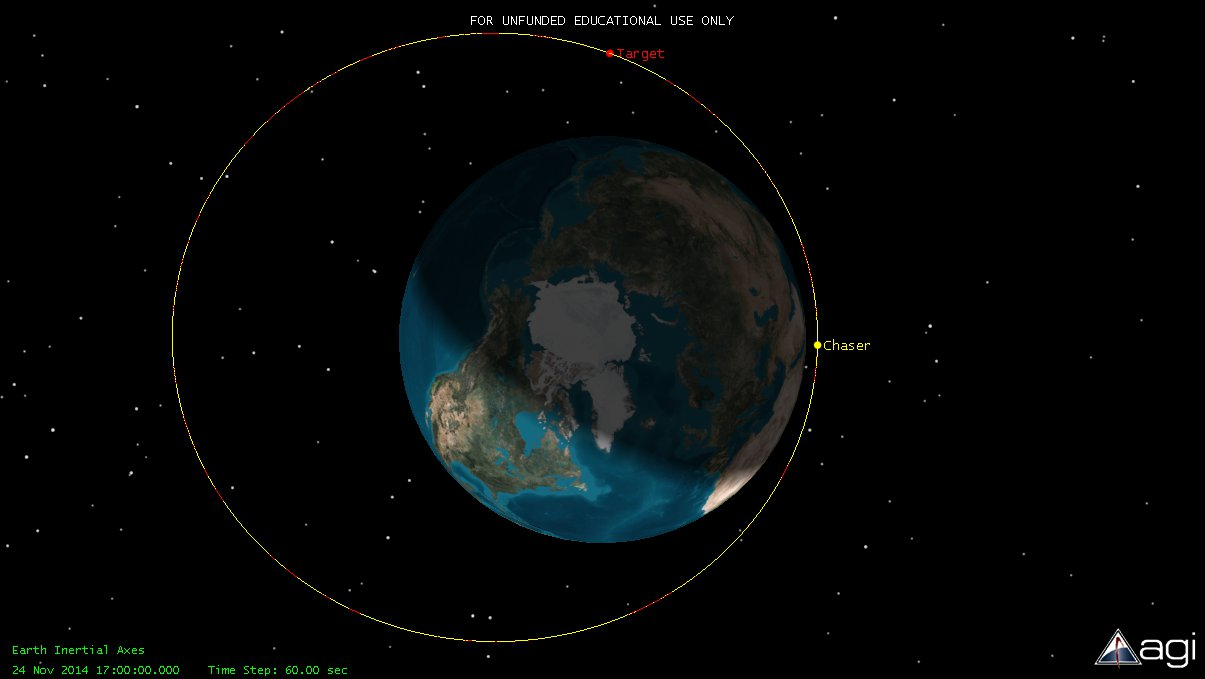
\includegraphics[width=0.9\textwidth]{Step4.eps}}
\caption{Step 4}
\end{figure}
\vfill
\begin{figure}
\centerline{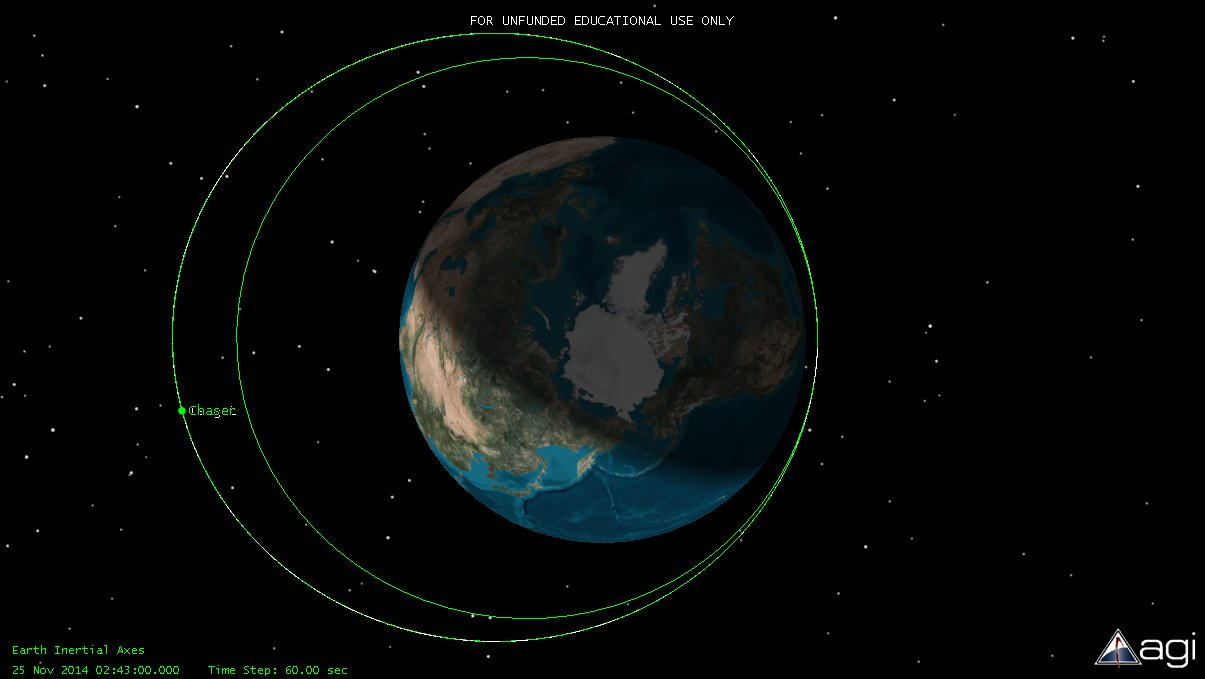
\includegraphics[width=0.9\textwidth]{Step7.eps}}
\caption{Step 8}
\end{figure}

\end{document}

